\documentclass[12pt]{article}

\usepackage{sbc-template}
\usepackage{graphicx,url}
\usepackage[utf8]{inputenc}
\usepackage[brazil]{babel}
\usepackage{float}
\usepackage{booktabs}
\usepackage{subcaption} 
\usepackage[labelformat=parens,labelsep=quad, skip=3pt]{caption}
     
\sloppy

\title{Predição de Falência Bancária\\usando Redes Neurais Artificiais}

\author{Helder Mateus dos Reis Matos\inst{1}}


\address{Faculdade de Computação -- Instituto de Ciências Exatas e Naturais\\ Universidade Federal do Pará (UFPA)\\
  Av. Augusto Correa 01, 66075-090 -- Belém, PA -- Brazil
  \email{helder.matos@icen.ufpa.br}
}

\begin{document} 

\maketitle

\begin{abstract}
This article describes the setup and use of an Artificial Neural Network (ANN) for a pattern classification problem. The problem is based on the prediction of bankruptcy using qualitative indicatives described by economic experts. The implementation, as well as the comparison between the different topologies tested are presented in order to justify the application of ANNs in the field of Economic Forecasting. During the creation of this paper some software tools were used, such as the numerical computing environment MATLAB R2015a and the programming language Python 3.8.
\end{abstract}

\begin{resumo}
Este artigo descreve a configuração e o uso de uma Rede Neural Artificial para um problema de classificação de padrões.
O problema consiste na predição de falência de sistemas bancários a partir de indicativos qualitativos descritos por especialistas em economia. A descrição da implementação, assim como a comparação das topologias desenvolvidas são apresentadas visando justificar o uso de RNAs no âmbito de previsão econômica. Foram utilizadas como ferramentas para a construção desta publicação o ambiente de computação numérica MATLAB 2015a e a linguagem de programação Python 3.8.
\end{resumo}


\section{Introdução}
Contexto.\\
Descrição do Problema.\\
Justificação do Artigo.\\
Objetivos.\\

\section{Fundamentação Teórica}
	\subsection{Avaliação Qualitativa}
	\cite{myoung:03}
	\subsection{Redes Neurais Artificiais}
	\cite{haykin}
	
\section{Experimentação}
	\subsection{Dataset - \textit{Qualitative Bankruptcy}}
	O conjunto de dados consiste em 250 amostras, com 7 atributos. Os seis primeiros atributos descrevem a avaliação qualitativa da amostra, onde são classificados de acordo com o seu grau de impacto, onde P, A e N indicam os graus positivo (positive), mediano (average) ou negativo (negativo), respectivamente. O último atributos tem os valores B (bankruptcy) e NB (non-bankruptcy) que indicam a classe na qual a amostra pertence, indicando falência ou não-falência, respectivamente.
	\begin{table}[H]
	\centering
	\caption{Atributos e Valores para o dataset \textit{Qualitative Bankruptcy}}
	\label{tab:exTable1}
	\begin{tabular}{ccc}
	\hline
	N & Atributos             & Valores       \\ \hline
	1 & Risco Industrial       & P, A, N \\
	2 & Risco de Gerenciamento       & P, A, N \\
	3 & Flexibilidade Financeira & P, A, N \\
	4 & Credibilidade           & P, A, N \\
	5 & Competitividade       & P, A, N \\
	6 & Risco Operacional        & P, A, N \\
	7 & Classe                 & B, NB   \\ \hline
	\end{tabular}
	\end{table}
	Valores de entradas em Redes Neurais Artificiais são assinalados como valores numéricos, reais ou inteiros. Entretanto, o conjunto de dados apresenta dados nominais que são facilmente interpretados em outras técnicas de aprendizado de máquina, como o de algoritmos genéticos usado por \cite{myoung:03}, mas que são ininteligíveis para RNAs. Portanto foi necessária uma transformação na atribuição dos valores nominais para numéricos, como mostrado na tabela 2.

	\begin{table}[H]
	\centering
	\caption{Valores Nominais transformados em Valores Numéricos}
	\label{tab:exTable2}
	\begin{tabular}{cc}
	\hline
	Valor Nominal & Valor Numérico \\ \hline
	P             & 4               \\
	A             & 3               \\
	N             & 2               \\
	B             & 1               \\
	NB            & 0               \\ \hline
	\end{tabular}
	\end{table}
	As 250 amostras foram divididas em três grupos: \textbf{amostras de treino} ($70\% = 176$ amostras) foram usadas para ajustar pesos e bias durante as épocas, \textbf{amostras de validação} (15$\% = 37$ amostras) foram usadas para reduzir o Erro Médio Quadrático (\textit{Mean Squared Error - MSE}), e  \textbf{amostras de teste} (15$\% = 37$ amostras) foram usadas para medir a performance da estrutura da rede.

	\subsection{Implementação da Rede Neural Artificial}
	A rede foi construída usando o \textit{Deep Learning Toolbox} disponível no MATLAB R2015a. O treino foi realizado usando as funções de ativação sigmóide (logsig) e tangente hiperbólica (tansig) nas camadas escondida e de saída, respectivamente. Como o problema é destinado a um problema simples de classificação de padrões, foi utilizado o algoritmo de Backpropagation de Levenberg-Marquardt.
	\begin{figure}[H]
	\centering
	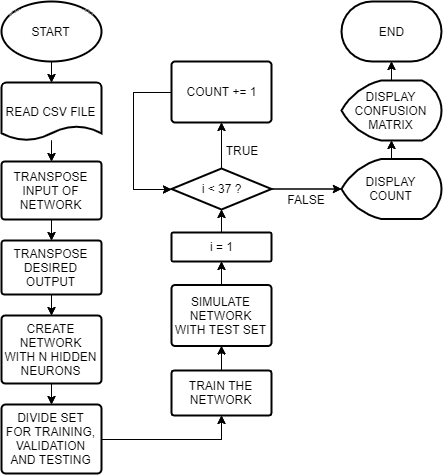
\includegraphics[width=.5\textwidth]{images/fig1.png}
	\caption{ANN Implementation Flowchart }
	\label{fig:exFig1}
	\end{figure}
	Four topologies were tested, with 5, 10, 15, and 30 neurons on the hidden layer.
\newpage
\section{Results}
	\subsection{Confusion Matrix Comparison}
	Analyzing the confusion matrix for all 4 topologies, it can be noticed that all of them achieve 100\% of success of prediction.

	\begin{figure}[H]
	\centering
	\begin{subfigure}{9cm}
	\centering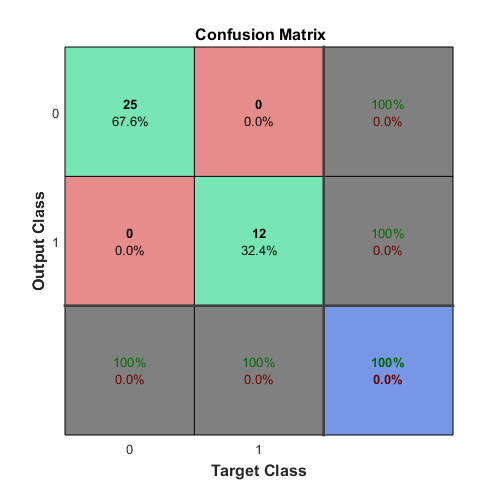
\includegraphics[width=9cm]{images/conf5_1.png}
	\caption{5 neurons on hidden layer}
	\end{subfigure}%
	\begin{subfigure}{9cm}
	\centering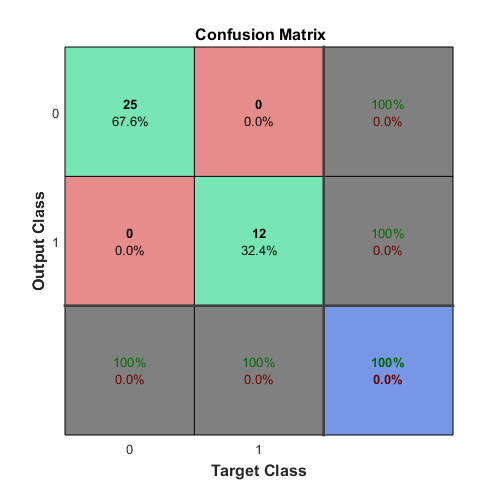
\includegraphics[width=9cm]{images/conf10_1.png}
	\caption{10 neurons on hidden layer}
	\end{subfigure}\vspace{10pt}
	 
	\begin{subfigure}{9cm}
	\centering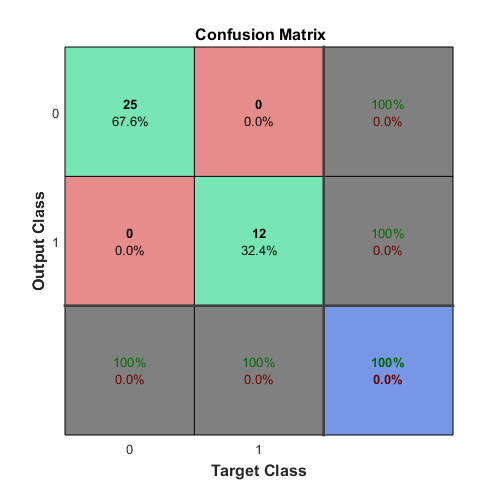
\includegraphics[width=9cm]{images/conf15_1.png}
	\caption{15 neurons on hidden layer}
	\end{subfigure}%
	\begin{subfigure}{9cm}
	\centering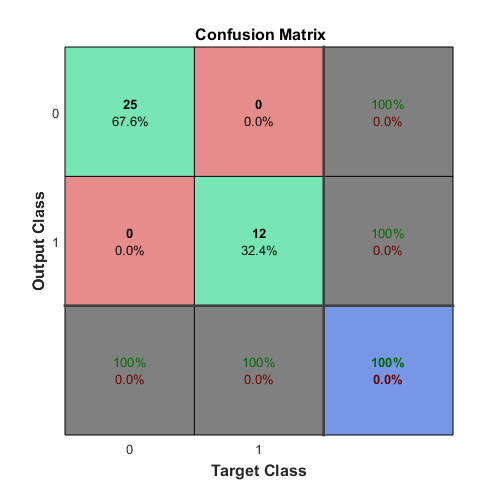
\includegraphics[width=9cm]{images/conf30_1.png}
	\caption{30 neurons on hidden layer}
	\end{subfigure}
	\end{figure}




\newpage
	\subsection{Performance Comparison}
	Analyzing the Best Validation Performance, the lowest value of the Mean Squared Error (MSE) was achieved with 15 neurons on the hidden layer. The topology with 30 neurons is satisfactory as well.
	
	\begin{figure}[H]
	\centering
	\begin{subfigure}{9cm}
	\centering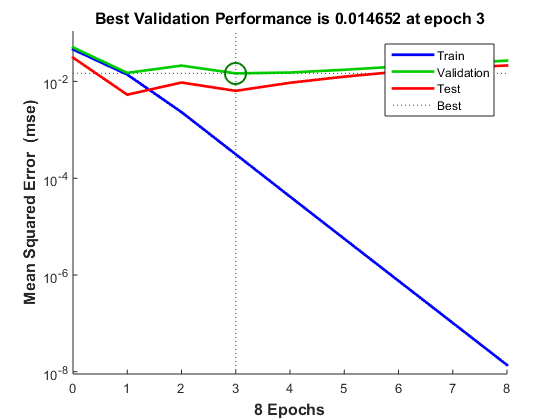
\includegraphics[width=9cm]{images/perf5_1.png}
	\caption{5 neurons on hidden layer}
	\end{subfigure}%
	\begin{subfigure}{9cm}
	\centering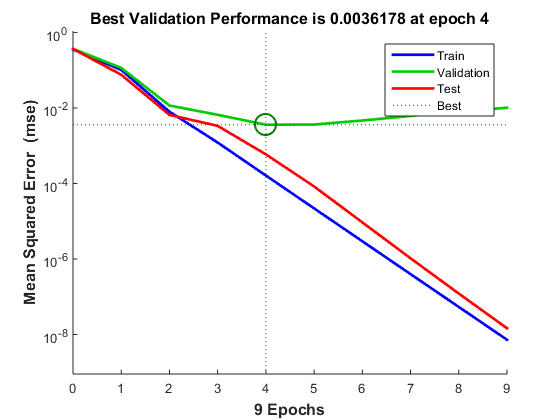
\includegraphics[width=9cm]{images/perf10_1.png}
	\caption{10 neurons on hidden layer}
	\end{subfigure}\vspace{10pt}
	 
	\begin{subfigure}{9cm}
	\centering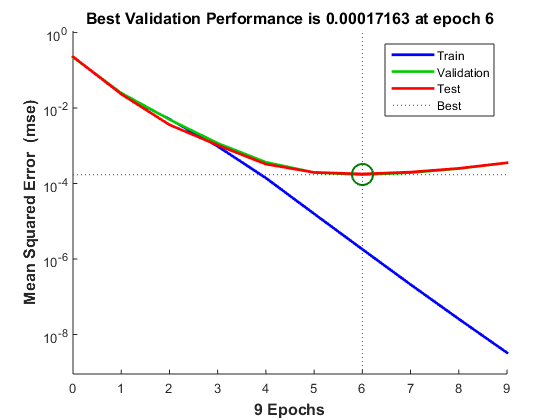
\includegraphics[width=9cm]{images/perf15_1.png}
	\caption{15 neurons on hidden layer}
	\end{subfigure}%
	\begin{subfigure}{9cm}
	\centering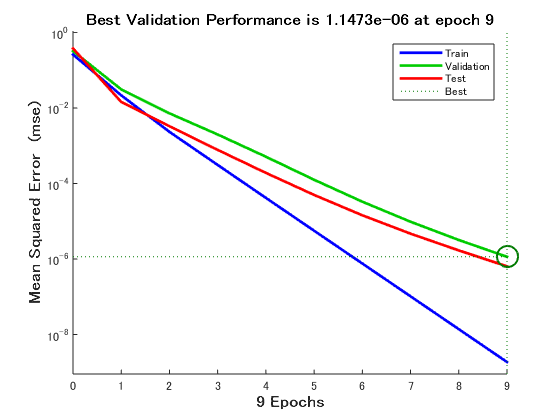
\includegraphics[width=9cm]{images/perf30_1.png}
	\caption{30 neurons on hidden layer}
	\end{subfigure}
	\end{figure}





\newpage
	\subsection{Regression Comparison}
	The ideal regression line must achieve a inclination of $45^{\circ}$ . The closest topology to $R = 1$ was achieved with 15 neurons.

	\begin{figure}[H]
	\centering
	\begin{subfigure}{9cm}
	\centering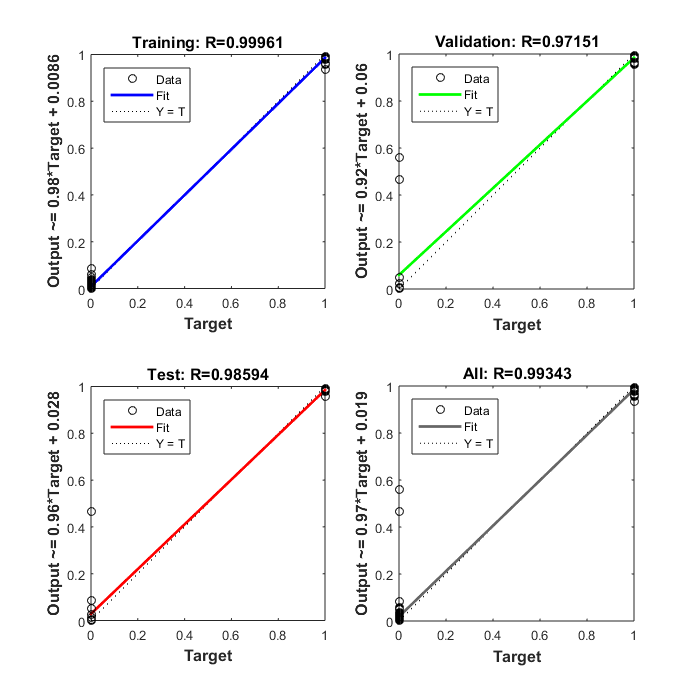
\includegraphics[width=9cm]{images/regression5_1.png}
	\caption{5 neurons on hidden layer}
	\end{subfigure}%
	\begin{subfigure}{9cm}
	\centering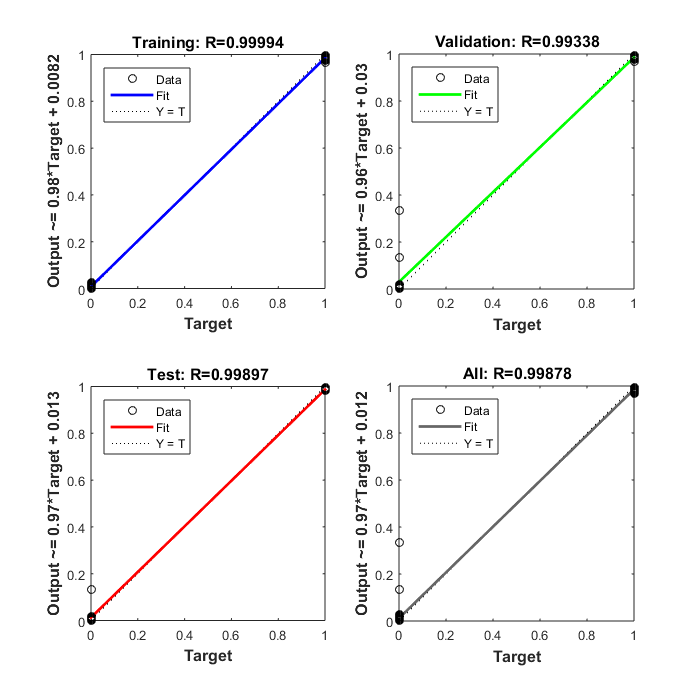
\includegraphics[width=9cm]{images/regression10_1.png}
	\caption{10 neurons on hidden layer}
	\end{subfigure}\vspace{10pt}
	 
	\begin{subfigure}{9cm}
	\centering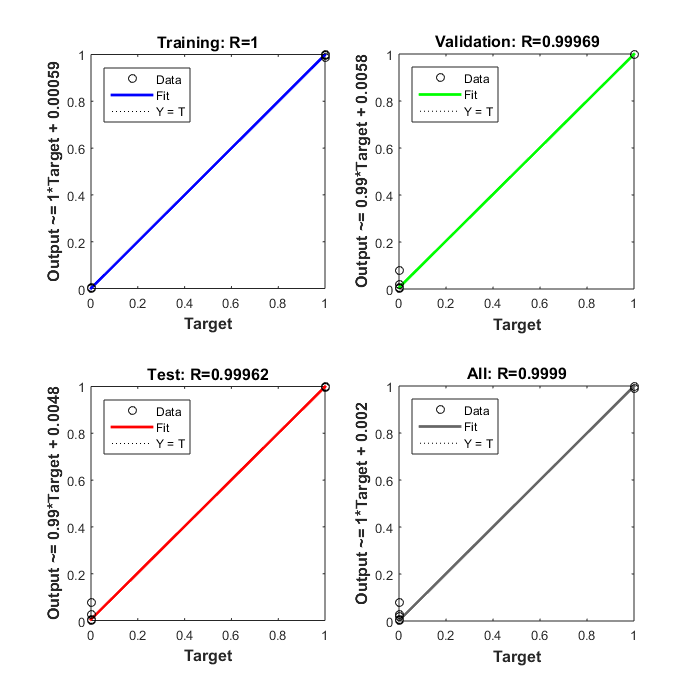
\includegraphics[width=9cm]{images/regression15_1.png}
	\caption{15 neurons on hidden layer}
	\end{subfigure}%
	\begin{subfigure}{9cm}
	\centering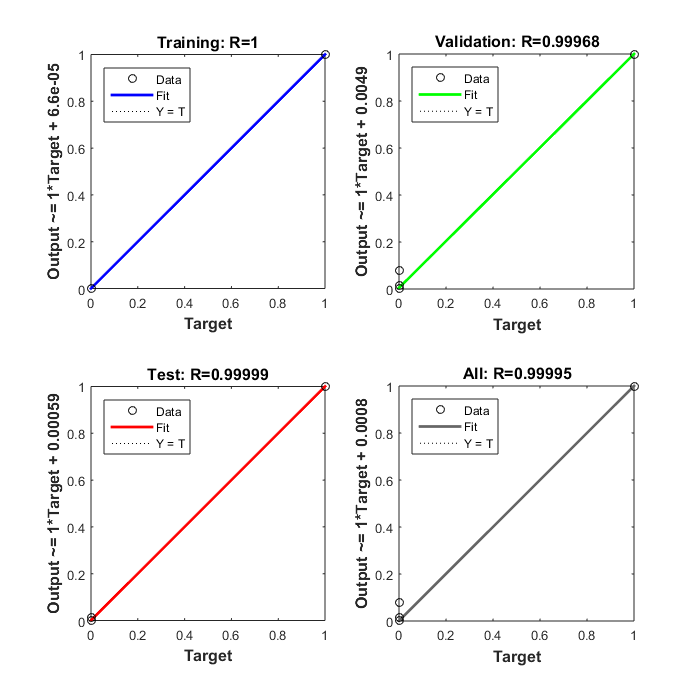
\includegraphics[width=9cm]{images/regression30_1.png}
	\caption{30 neurons on hidden layer}
	\end{subfigure}
	\end{figure}

\newpage
\section{Conclusion}
	The topology using 15 neurons on the hidden layer managed to satisfy three comparison parameters, which proved that Artificial Neuron Networks can be used to approximate statistical behavior in economics. 
	Some improvements can be achieved, such as training the same topology more than once, testing with different neurons on the hidden layer, using different transfer functions and convert nominal values into numerical using One-Hot Encoding, which would provide even more accurate results.


\bibliographystyle{sbc}
\bibliography{sbc-template}

\end{document}
